Tunnistautumisessa on kolme osapuolta: asiakasohjelma, web-palvelu ja tunnistautumispalvelu. Osapuolet on esitetty kuvassa \ref{composition}, jossa on mukana myös tunnistautumispalvelun käyttämä käyttäjänhallinta. Käyttäjähallinta voi olla myös osa tunnistautumispalvelua tai oma komponenttinsa, tunnistautumisen kannalta sillä ei ole väliä.

\begin{figure}[ht]
\centering
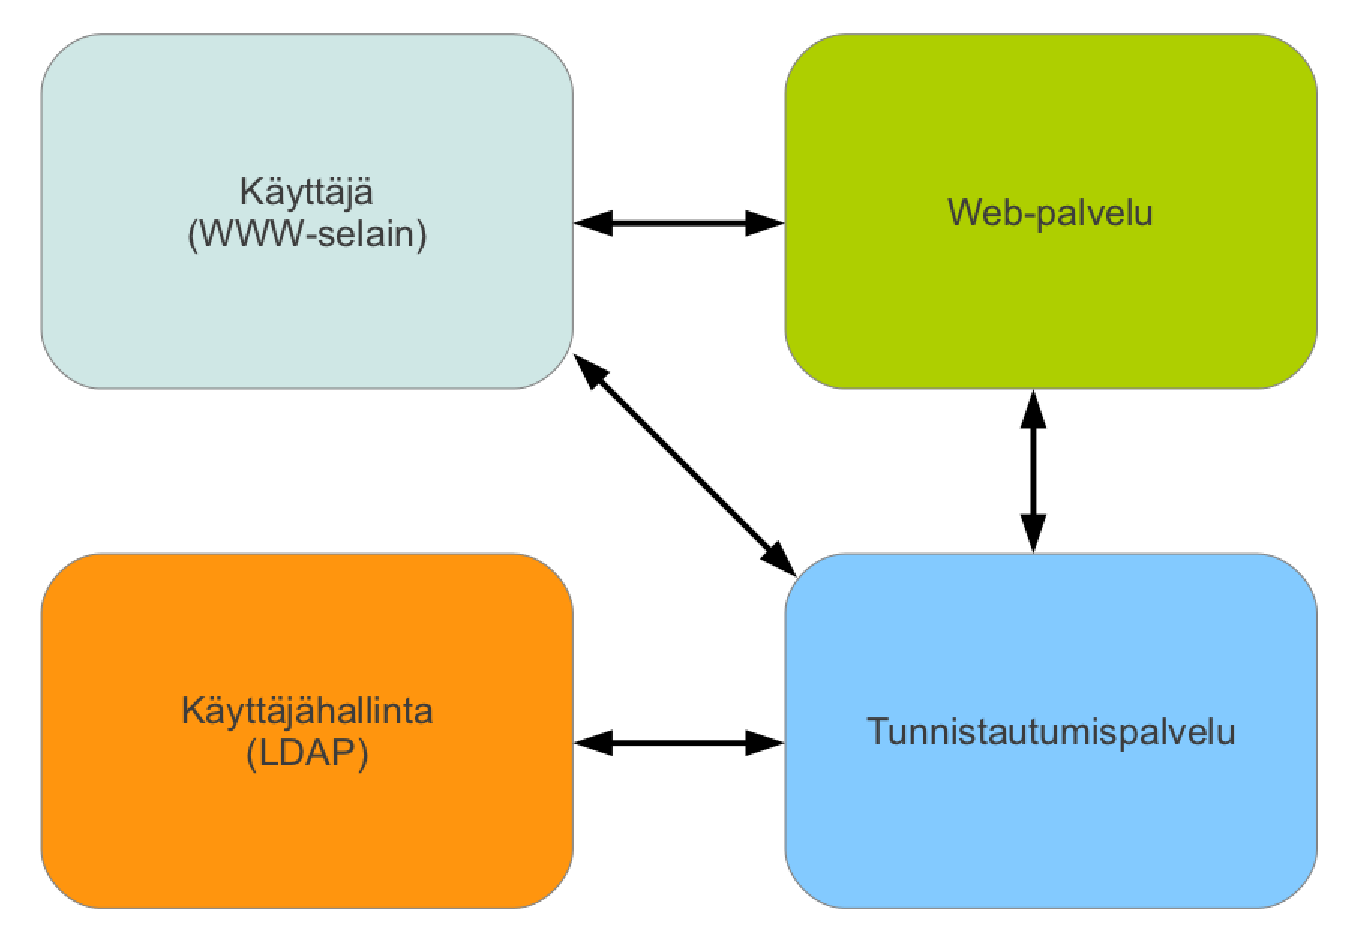
\includegraphics[width=0.7\textwidth]{teknologiat/composition.eps}
\caption{Keskitetyn tunnistautumisen osapuolet.}%
\label{composition}
\end{figure}

Kuvassa \ref{oauth} on tunnistautumisprotokollien sekvenssikaavio, jossa on kuvattu vaiheet käyttäjän kirjautuessa web-palveluun. Ensimmäiseksi käyttäjä menee asiakasohjelmalla web-palveluun, joka pyytää tunnistautumista erillisessä tunnistautumispalvelussa. Käyttäjän asiakasohjelma ohjataan tunnistautumispalvelun sivulle, joka on yhteydessä organisaation käyttäjähallintaan. Jos käyttäjähallinnasta löytyy käyttäjän syöttämät tunnistetiedot, palautetaan käyttäjälle valtuutusavain, jonka käyttäjä lähettää takaisin web-palvelulle \cite{nisti}. Tämän jälkeen web-palvelu varmistaa tunnistautumispalvelulta valtuutusavaimen oikeellisuuden ja tunnistautumispalvelu palauttaa käyttäjän tiedot web-palvelulle \cite{nisti}.

Useimmat vaiheista tapahtu käyttäjältä näkymättömissä selaimen uudelleenohjauksella. Käyttäjälle näkyvät vaiheet ovat 4 ja 5, joissa käyttäjältä pyydetään käyttäjätunnus ja salasana sekä varmistetaan tietojen lähetys web-palveluun. Käyttäjän syötettä vaativat vaiheet on esitetty aiemmassa kuvassa \ref{facebook_login}.

\begin{figure}[ht]
\centering
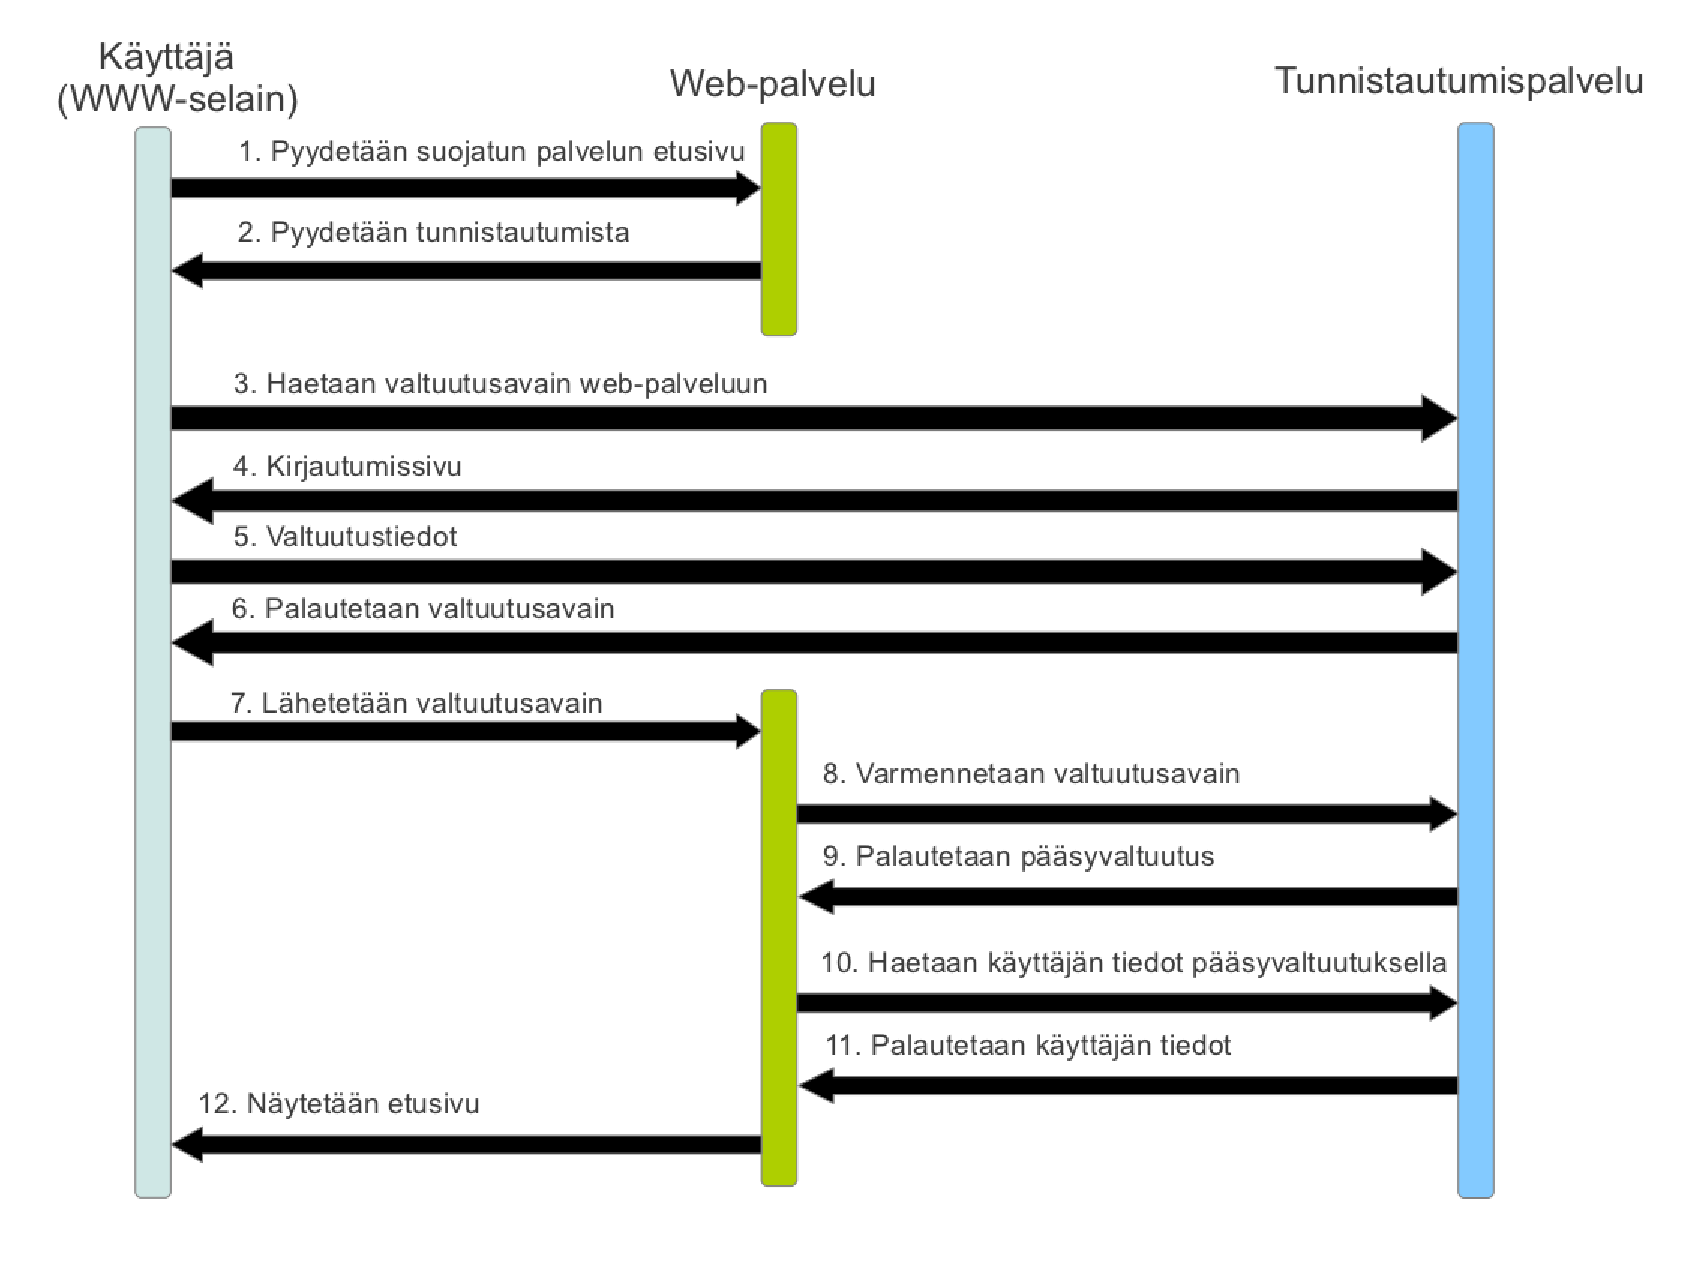
\includegraphics[width=\textwidth]{teknologiat/protokollat/oauth.eps}
\caption{Tunnistautuminen sekvenssikaaviona.}%
\label{oauth}
\end{figure}